% !TEX root = ../lectures_olympics.tex

\chapter{牛顿运动定律及应用}

\section{三大运动定律}
质点是对运动物体的简化模型,它的运动学性质集中体现为它做为点的一面,可以用质点的位置随时间的变化关系给出,在运动学的学习中已经广泛讨论了质点和由多个质点构成的质点系统的运动。
与此同时质点还具有质量,质量是物体的一个基本属性,这一点在初中的课程中已经学过,对于均匀的物质来说它的质量由物质的密度和体积的乘积共同决定;如果一个物体由多个部分组成,则其质量为组成它的各个部分质量的和。

当质点运动在空间中运动时,具有相同速度但不同质量的质点所表现出的性质也大不相同,为了体现这种不同,定义一个新的物理量--\emph{动量},它是一个矢量,定认为质点的质量和速度的乘积,方向则与运动质点的速度方向相同:
\begin{equation}\label{eqn: newton-definition-of-momentum}
\vec{p} = m\vec{v}.
\end{equation}
在外力作用下,质量越大的物体运动状态的变化越不明显,反之当力作用于质量较小的物体时,则会引起巨大速度变化。

在大量经验和实验的基础上,英国物理学家牛顿给出了支配物体运动的三大定律,它们分别是
\begin{description}
\item[第一定律]
不受外力作用的物体必将保持静止或作匀速直线运动。
\item[第二定律]
受到外力的物体将作加速运动,其动量随时间的变化率等于所受的外力。
\item[第三定律]
任意两个物体之间的相互作用力大小相等、方向相反并且在一条直线上。
\end{description}
牛顿的三个运动定律是动力学的基础,相当精确地给出了物体的宏观物体的运动规律。
作为最基本的运动定律,有必要深入地讨论它们适用的条件、分析它们所带来丰富的对自然现象的理解。

\subsection{第一定律:惯性}
牛顿第一定律又被称为\emph{惯性定律},指出在不受任何影响状态下自然界中各个物理“应有”的运动状态,即我们在运动学中见过的最简单的运动--匀速直线运动。
惯性是任何物体所固有的属性,它使得物体都有一种内在的抵抗外力,而保持其原有运动状态,也就是运动速度的趋势。
惯性本身也是可以度量的,物体惯性大小的量度不是别的,正是它本身的质量。
质量越大的物体惯性越大,反之就越小,在相同力的作用下,质量大的物体运动状态的改变反而越小,这和我们的日常经验也是一致的。

在运动学中可以在任意的参考系中建立合适的坐标系来描写所有物体的运动,但到了动力学中这个事实就不再成立。
牛顿定律并不能够应用到所有的参考系中,而只能是一类极其特殊的参考系,称做\emph{惯性参考系}或\emph{惯性系},只有在惯性系当中,那些不受力物体的运动才是匀速直线运动。
惯性系的选取并不唯一,可以通过运动学的事实证明,当参考系$S$的确为惯性系时,所有相对于$S$作匀速直线运动的参考系其实都是惯性系。
同一个不受力质点在不同的惯性系中均作匀速直线运动,只不过在不同的惯性系中的运动速度有所不同。
但是那些相对于$S$作加速度运动的参考则无一例外都不是惯性系,因为不同参考系中加速度的变换关系告诉我们,当一个质点相对于$S$匀速运动时,它在新的参考系中的加速度必然不为零,牛顿第一定律不再成立,将不再是惯性参考系。

关于是否存在真正的惯性参考系,在哪里才能够找到惯性系在很长时间以来都是极具争论的话题。
绝大多数力学现象都是以地球表面为参考系来描写的,实践上在地表参考系中应用牛顿定律可以在相当高的精度上描写物体的运动,但对于那类运动范围较广、速度较快或观测精度较高的运动过程来说,地表则不能够当做惯性系来看待。
我们知道,地球不但有自转,也有围绕太阳的公转,这些转动都使得地球其实不能够当做严格的惯性系。
当以太阳为参考系时牛顿定律能够在更高的精度上成立,但天文观测事实也表明,太阳带着所有太阳系中的天体实际上以极高的速度围绕银河系中心旋转,虽然加速度很小,但也不是严格意义上的惯性参考系。
关于惯性系各个方面的争论始终存在,爱因斯坦的相对论给出了部分答案,但也受到来自宇宙学的挑战。
在实践上,如没有特别说明,当描写地球上的物理过程时均取地表为惯性参考系,而那些相对于地面作加速运动的参考系则是非惯性系。

【思考】你能够发挥想象力或通过已知的物理知识给出一个惯性参考系吗?


\subsection{第二定律:加速}
第一定律指出,不受力的物体在惯性系中运动速度不会发生变化,而第二定律进一步告诉我们当物体受到力的作用时其运动状态是如何发生变化的。
在相同外力作用下不同物体运动的变化不尽相同,利用前面引入的动量,第二定律可以写成
\begin{equation}
F = \lim_{ \Delta t\rightarrow 0} \frac{ \Delta p}{ \Delta t}
\end{equation}
因为在牛顿力学研究范围内大部分物体在运动过程中的质量变化总是很小,根据动量的定义\ref{eqn: newton-definition-of-momentum} 牛顿第二定律也可以写为更著名的形式
\begin{equation}
\vec{F} = \frac{ \Delta (m\vec{v})}{ \Delta t} = m \frac{ \Delta\vec{v}}{ \Delta t} = m\vec{a}.
\end{equation}\label{eqn: newton-f=ma}
即运动物体的加速度与其自身质量的乘积在数量上等于它所受的外力,并且加速度的方向与外力方向相同,这将是我们今后一段时间更为常用的第二定律表达式。
关于牛顿第二定律的使用有几点需要特别注意的地方
\begin{itemize}
\item
和第一定律一样,牛顿第二定律也只有在惯性系中才成立。
对于非惯性参考系,第二定律必须经过改写才能够适用。
\item
第二定律只适用于宏观低速运动的物体,当物体的运动速度与光速接近,或者对于质量极小的微观粒子,例如原子和构成原子的更小的粒子牛顿定律则不再成立,它们的运动变化满足其它的物理定律,我们将在随后的课程中学习。
\item
当一个物体受到多个力同时作用时,它的加速度由所受所有力的合力所决定,而合力则是各个力的矢量和。
\end{itemize}

【思考】牛顿第一定律是否仅仅是第二定律在$F=0$时的特例?

第二定律有两大类典型的应用,它们分别是通过观察到物体的真实运动进而确定物体所受外力的性质,以及在已知运动物体所受所有外力时,预测该物体未来的运动行为。

研究物体运动的早期是通过观察各个物体的运动利用第二定律推测其所受外力的大小和方向与物体的性质、外界情况的关系。
在运动学中我们曾经广泛地讨论了多种运动形式,通过牛顿定律可知,造成千变万化的运动的原因是由于物体受到力的作用,并且质量为$m$的物体在作给定形式运动时,它所受到的力必然就是它的质量与各个时刻加速度的乘积。
通过分析运动过程,可以得到多种情况下的受力,例如
\begin{itemize}
\item
地表附近抛出物体均做抛体运动,加速度大小均为重力加速度$g$,指向地面。
根据牛顿定律,所有地表附近质量为$m$的物体在飞行过程中时刻受到大小
\begin{equation}
F = mg
\end{equation}\label{eqn: motion-f=mg}
指向地面的力,这就是熟知的\emph{重力}。
所有的物体均为受到重力作用,方向竖直向下,而作用点则是物体的重心。
\item
匀速圆周运动的物体虽然速率时刻保持不变,但是由于速度方向不断地发生变化,各个时刻都有指向圆心的向心加速度。
当质量为$m$的质点线速度为$v$作半径为$R$匀速圆周运动时,必须时刻受到指向圆心,大小为
\begin{equation}
F = m \frac{v^2}{R}
\end{equation}
力的作用,因为这时受力时刻指向圆心,所以将其形象地称做\emph{向心力}。
如果没有向心力,那么质点则不可能做圆周运动,而是按照第一定律告诉我们的那样沿直线运动。

\item
太阳系的各个行星运动均满足开普勒三定律,通过对行星运动的分析可知,轨道上的行星所受的力时刻指向太阳(开普勒第二定律),大小正比于行星的质量,反比于行星到太阳的距离。
在这些结论的基础上牛顿又进行了大胆的假设,最终得到了著名的\emph{万有引力},任意两个物体之间都有指向对方的引力作用,大小正比于两物体的质量$m_{1,2}$,反比于距离$r$的平方
\begin{equation}
F = G \frac{m_1m_2}{r^2}.
\end{equation}
万有引力是牛顿力学最光辉的成就之一,在随后的学习中将专门对其进行讨论。
\item
当物体的运动受到约束时会受到\emph{约束力}。
和重力、弹簧弹力等不同的是,约束力的大小和方向并不能够在一开始就决定下来,会随着受约束物体所受其它力和运动状态有关。
典型的约束力有平面的弹力、连轩内的弹力、绳子的拉力等等,相当一部分问题的复杂性来自于约束力,需要在运动的不同时刻确定约束力进而判断物体的运动。
\item
自然界中还广泛地存在有各种形式的阻力作用,它们会降低机械的效率,增加预测运动的难度。
典型的阻力包括当两物体相互接触且有相对运动或相对运动趋势时的滑动或静\emph{摩擦力},通过观察发现滑动摩擦力通常正比于两物体之间的压力$N$,与相对运动方向相反,比例系数则被称做\emph{摩擦系数$\mu$},与相互接触物体的性质有关:
\begin{equation}
f = \mu N.
\end{equation}
除了来自于接触的阻力以外,水中或空气中运动物体也会受到阻力,来自于流体的阻力非常复杂,由流体的性质、运动物体的形状和速度共同决定,很难定量地给出。
将来会在一些理想化的情况下讨论流体阻力的性质。
\end{itemize}


%%%%%%%%%%%%%%%%%
\begin{example}

一个质量为$m$,沿平面上$x$轴运动质点的位置随时间的关系为
\[
x(t) = A\cos\omega t,
\]
求它所受到外力随位置的关系。
\tagged{student}{\vspace*{4cm}}
\begin{taggedblock}{teacher}
\newline
解析:在运动学中已经知道,当运动方程为由上式给出时,它的加速度
\[
a = -\omega^2 A \cos\omega t = -\omega^2 x,
\]
根据牛顿第二定律可知它所受的外力为
\[
F(x) = ma = -m\omega^2 x,
\]
可以看出它正比于质点离开原点的距离并且与位移方向相反,指向坐标系原点。
\end{taggedblock}
\end{example}
%%%%%%%%%%%%%%%%%%%%%%


%%%%%%%%%%%%%
\begin{example}
	在一固定平面上一个质点的运动由方程
	\[
		x(t)=A\cos\omega t, \qquad y(t)=A\sin\omega t
	\]
	给出,求它在运动过程中的受力。
	\tagged{student}{\vspace*{4cm}}
	\begin{taggedblock}{teacher}
	\newline	
		解析:
	\end{taggedblock}
\end{example}
%%%%%%%%%%%%%%%%%%%%

%%%%%%%%%%%%%
\begin{example}
	一个物体受何种力可以使其沿着
	\[
	x(t)=A\cos\omega t, \qquad y(t)=A\sin\omega t,\qquad z(t)=v(t)
	\]
	所给出的轨道运动?
	\tagged{student}{\vspace*{4cm}}
	\begin{taggedblock}{teacher}
\newline	
		解析:
	\end{taggedblock}
\end{example}
%%%%%%%%%%%%%%%%%%%%

%%%%%%%%%%%%%%%%%
\begin{example}

在一个研究质点在特定介质中运动所受阻力的实验中发现,一个质量为$m$初速度为$v_0$的质点在阻力作用下减速,且速度随它在介质中前进的距离正成比。
合理地建立坐标系,可以将其速度表达为
\[
v(x) = v_0 - \alpha x,
\]
探讨它所受阻力的形式。
\tagged{student}{\vspace*{4cm}}
\begin{taggedblock}{teacher}
\newline
解析:将加速度的表达式稍做变形可得:
\[
a = \frac{\Delta v}{\Delta t} = \frac{\Delta v}{\Delta x}\frac{\Delta x}{\Delta t} = \frac{\Delta v}{\Delta x}v,
\]
根据已知条件可得
\[
\frac{\Delta v}{\Delta x} = -\alpha,
\]
这样将加速度的表达式代入牛顿第二定律当中可得:
\[
F = ma = -\alpha m v
\]
可见它所受阻力与速度方向相反,正比于速度的大小。
\end{taggedblock}
\end{example}
%%%%%%%%%%%%%%%%%%%%%%

力学中很多的分支都是从对运动物体的观察开始,进而找到在特定环境下相互作用力的特点,通过牛顿定律预测将来的运动并与测量相比较最终确信其正确性,最后得到可靠的结论并应用于实践。
在已知力的性质以后就可以利用第二定律计算未来的运动。
因为当质量为$m$的运动物体在某一时刻的位置$\vec{r}$、速度$\vec{v}$和所受外力$\vec{F}$均为已知时,此时它运动的加速度就是
\begin{equation}
\vec{a} = \frac{\vec{F}}{m},
\end{equation}
在极小的时间间隔$ \Delta t$里,近似地认为它的速度和受力的变化可以忽略不计,这样在$ \Delta t$时间之后它的位置、速度的变化量分别为
\begin{equation}
\Delta \vec{r} = \vec{v} \Delta t,\qquad \Delta \vec{v}  = \frac{\vec{F}}{m} \Delta t
\end{equation}
也就是说它位置和速度的变化量都能够计算出来。
只要知道它在新的位置和新的速度下的受力的大小,前面的过程就可以不段地重复,最后就能够预测将来任意时刻的位置和速度!

从第二定律当中可以看出,在恒力作用下物体将做匀加速运动,加速度的大小等于力与运动质点质量的比值,方向则与力的方向一致。
匀加速运动在过去运动学的学习中已经广泛地研究,所以只需要对运动物体做完整、无遗漏的受力分析,就可以确定它的加速度,进而得到它在受力作用下的运动。
如果所受外力并非恒力,就像引力那样时则必须用到全新的数学工具--微积分才能够处理这类问题;事实上微积分的出现也正是牛顿在尝试解决引力作用下物体运动问题的推动下被发明的。
接下来我们就从相对简单的问题出发,分析外力作用下物体运动的性质,将所得到的结论和方法应用到越来越复杂的系统当中,并尝试找到研究这类问题一般的方法。






%%%%%%%%%%%%%%%%%
\begin{example}

一个质量为$m$的质点在恒力$F$作用下沿直线加速运动,经过一段时间它的速度由$v_0$变成了$v_1$,求外力作用的时间以及外力作用下质点的位移。
\tagged{student}{\vspace*{4cm}}
\begin{taggedblock}{teacher}
\newline
解析:设外力作用的时间为$\Delta t$根据已知的条件可知运动的加速度
\[
a = \frac{v-v_0}{\Delta t}
\]
根据牛顿定律可知
\[  F = ma = m\frac{v_1-v_0}{\Delta t},\qquad \Delta t = \frac{m(v_1-v_0)}{F}\]
\end{taggedblock}
\end{example}
%%%%%%%%%%%%%%%%%%%%%%



%%%%%%%%%%%%%%%%%
\begin{example}

证明:任意恒力作用下质点运动的轨迹均为抛物线,且开口指向恒力的方向。
\tagged{student}{\vspace*{4cm}}
\begin{taggedblock}{teacher}
\newline
解析:略
\end{taggedblock}
\end{example}
%%%%%%%%%%%%%%%%%%%%%%


%%%%%%%%%%%%%
\begin{example}
	一个质量为$m$的质点在一平面内运动,开始时刻其运动速度为$v$,在此后的运动过程中它时刻受到一个与速度方向垂直,指向前进方向右侧且大小不变的力的作用,大小为$F$。
	试根据牛顿第二定律给该质点的运动轨迹,如果在外力作用下该质点做周期运动的话,请给出运动的周期与已知变量的关系。
	\tagged{student}{\vspace*{4cm}}
	\begin{taggedblock}{teacher}
\newline
		解析:该质点做圆周运动
		\[a=\frac{F}{m}=m\frac{v^2}{r}\]
		\[2\pi*r=vT\]
	\end{taggedblock}
\end{example}
%%%%%%%%%%%%%%%%%%%%






\subsection{第三定律:相互作用}
第三定律看似平淡无奇,而且并不像前两个定律那样普遍,但其实在力学中它对于分析问题来说却是必不可少的;另外当深入地分析三大定律之间的内在关系时也会发现第三定律其实在里面扮演着非常重要的角色。
它告诉我们任意两个物体之间相互作用的性质:大小相等、方向相反并且在一条直线上,利用它可以在已知部分受力的情况下准确地找出多个物体之间受力的关系。
从某种意义上讲万有引力定律的出现正是建立在牛顿第三定律基础上的,地球在太阳引力作用下做椭圆轨道运动,而与此同时地球也以相同的力吸引太阳,只不过因为太阳的质量远大于地球的质量,所以在相同力作用下的加速度很小而已。

【思考】事实上牛顿第三定律给出了质量严格且具有可操作性的定义,你能够独立地找到它吗?

%%%%%%%%%%%%%
\begin{example}
	如图所示,光滑水平面上两个质量分别为$m_1$、$m_2$的物体$A、B$由不可伸长且质量可忽略不计的绳连接,有一个大小和方向均不变的力$F$作用于$A$,求两物体的加速度。
	\begin{flushright}
		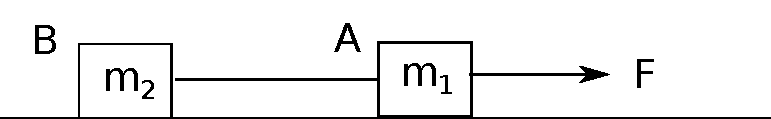
\includegraphics[width = 0.4\textwidth]{images/newton-11.pdf} 
	\end{flushright}
	\tagged{student}{\vspace*{4cm}}
	\begin{taggedblock}{teacher}
		\noindent
		解析:引入整体分析的方法
	\end{taggedblock}
\end{example}
%%%%%%%%%%%%%%%%%%%%

%%%%%%%%%%%%%%%%%
\begin{example}

如图,质量分别为$m$和$M$的物体放在光滑水平面上,现有一恒定大小的外力$F$作用于$M$,两物体之间接触面不光滑,摩擦系数为$\mu$,求两个物体的加速度。
\begin{flushright}
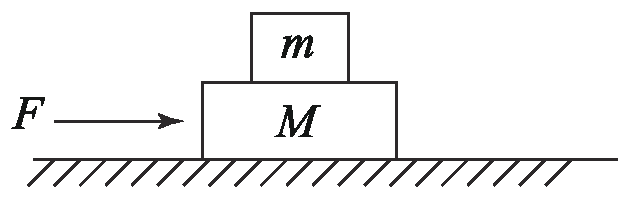
\includegraphics[width = 0.4\textwidth]{images/newton-6.pdf} 
\end{flushright}
\tagged{student}{\vspace*{4cm}}
\begin{taggedblock}{teacher}
\noindent
解析:要注意两种情况
\end{taggedblock}
\end{example}
%%%%%%%%%%%%%%%%%%%%%%


%%%%%%%%%%%%%%%%%
\begin{example}

两个质量分别为$m_{1,2}$的物体由无摩擦的滑轮连接如图放置,已知$m_2>m_1$,求两者的加速度。
\begin{flushright}
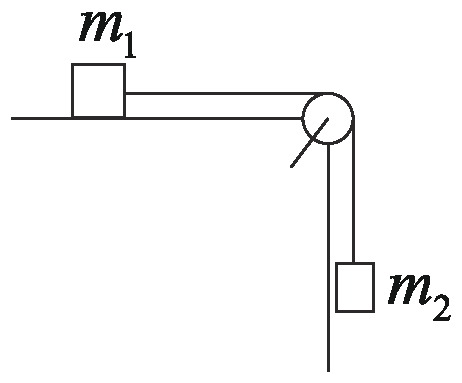
\includegraphics[width = 0.4\textwidth]{images/newton-7.pdf} 
\end{flushright}

\tagged{student}{\vspace*{4cm}}
\begin{taggedblock}{teacher}
\noindent
解析:加速度大小相同
$a=\frac{m_2g}{m_2+m_1}$
\end{taggedblock}
\end{example}
%%%%%%%%%%%%%%%%%%%%%%

\section{应用}

将牛顿三定律与受力对象的性质和特点有机地结合在一起可以解决几乎所有物体在受力作用下的运动问题,但是随着相互作用物体的增加、系统本身的复杂性的提升,预测运动将变得越来越复杂。
物体在受力作用下运动的问题将贯穿整个物理学,我们将从简单的问题开始掌握一般的技术,随着时间的推移你将能够解决越来越多、越来越复杂的问题。


%%%%%%%%%%%%%
\begin{example}
	地球的半径约为$6.4\pow{3}\unit{km}$,地表附近重力加速度为$9.8\unit{m/s^2}$;通过天文观测发现月球的公转轨道平均半径约为$3.8\pow{5}\unit{km}$,公转周期约为27.3天。
	传说牛顿在被苹果砸到以后开始考虑导致地球表面物体下落和月球的公转是同一种力,你能否通过上面的数据给出月球公转加速度与地球表面重力加速度的关系吗?
	\tagged{student}{\vspace*{4cm}}
	\begin{taggedblock}{teacher}
		\newline
		解析:月球公转加速度与地球表面重力加速度之比,是月球公转半径平方与地球半径平方之比的导数
	\end{taggedblock}
\end{example}
%%%%%%%%%%%%%%%%%%%%



%%%%%%%%%%%%%%%%%
\begin{example}
质量分别为$m_1$和$m_2$的两个小物块用轻绳连结,绳跨过位于倾角$\alpha=30^\circ$的光滑斜面顶端的轻滑轮,滑轮与转轴之间的磨擦不计,斜面固定在水平桌面上,如图所示。
第一次,$m_1$悬空,$m_2$放在斜面上,用$t$表示$m_2$自斜面底端由静止开始运动至斜面顶端所需的时间。
第二次,将$m_1$和$m_2$位置互换,使$m_2$悬空,$m_1$放在斜面上,发现$m_1$自斜面底端由静止开始运动至斜面顶端所需的时间为$t/3$。
求$m_1$与$m_2$之比。
\begin{flushright}
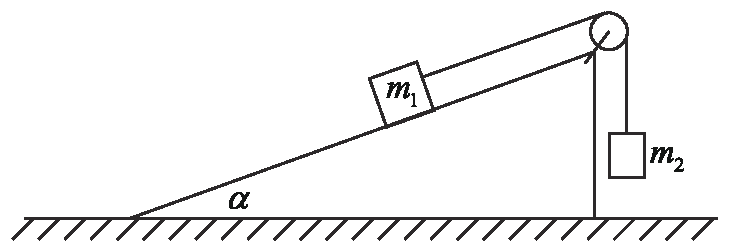
\includegraphics[width = 0.4\textwidth]{images/newton-5.pdf} 
\end{flushright}

\tagged{student}{\vspace*{4cm}}
\begin{taggedblock}{teacher}
\noindent
解析:
$\frac{m_1}{m_2}=\frac{11}{19}$
\end{taggedblock}
\end{example}
%%%%%%%%%%%%%%%%%%%%%%




%%%%%%%%%%%%%%%%%
\begin{example}
	
	一个质点自倾角为$\alpha$的斜面上方定点$A$,沿光滑斜槽从静止开始滑下,为了使质点在最短时间到达斜面,求斜槽与竖直方向的夹角$\beta$应等于多少?
	\begin{flushright}
		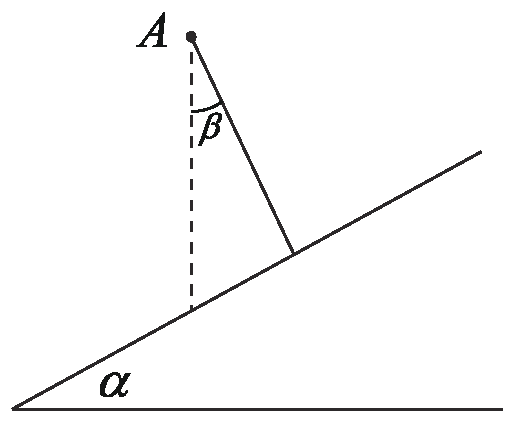
\includegraphics[width = 0.4\textwidth]{images/newton-10.pdf} 
	\end{flushright}
	\tagged{student}{\vspace*{4cm}}
	\begin{taggedblock}{teacher}
		\noindent
		解析:
		$\beta=\frac{\alpha}{2}$
	\end{taggedblock}
\end{example}
%%%%%%%%%%%%%%%%%%%%%%

在系统中包含有摩擦力时要格外小心,先前我们知道两固体表面之间的滑动摩擦力正比于相互之间的压力,比例系数称为摩擦系数;如果两物体保持相对静止且有相对运动趋势的话则有静摩擦力的作用,静摩擦力的性质由最大静摩擦系数给出,它的大小总是介于零到最大静摩擦力之间。
当在包含摩擦力的问题中分析物体运动时要注意当所有物体所处的环境为已知时,通常需要做一个判断以确定相互摩擦的两个物体之间究竟有无相对运动才能够进一步地使用牛顿定律进行分析。
在有些情况下,当两物体的速度在摩擦力作用下发生变化或外力发生改变时,两种状态之间还可能发生转化,这时相对运动状态变化时各个物体的运动状态对于我们来说就非常关键了。

%%%%%%%%%%%%%%%%%%%%%%%%%%%%%%%%%%
\begin{example}
一质量为$M$的平顶小车,以速度$v_0$沿水平的光滑轨道作匀速直线运动。
现将一质量为$m$的小物块钱无初速度地放置在车顶的前缘。
已知物块和车顶之间的滑动摩擦系数为$\mu$,若要求物块不会从车顶后缘掉下,则该车顶长度至少要多少?
\begin{flushright}
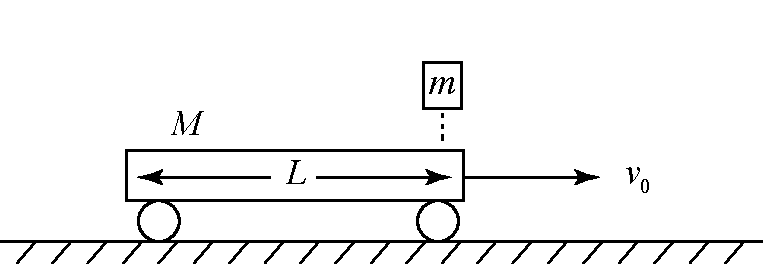
\includegraphics[width=0.5\textwidth]{images/newton-problem-1.pdf}
\end{flushright}
\tagged{student}{\vspace*{4cm}}
\begin{taggedblock}{teacher}
\noindent
解析:
$L=\frac{Mv_0^2}{2g\mu(m+M)}$
\end{taggedblock}
\end{example}
%%%%%%%%%%%%%%%%%%%%%%%%%%



%%%%%%%%%%%%%%%%%
\begin{example}

质量$m=1.5\unit{kg}$的物块在水平恒力$F$作用下从水平面上$ A $点由静止开始运动,运动一段距离之后撤去该力,物块继续滑行$ t=2.0\unit{s} $后停在$ B $点,已知$ A,B $两点点的距离$x = 5.0\unit{m}$,物块与水平面之间的动摩擦系数$ \mu = 0.20 $,求恒力$ F $的大小,简单起见取$g = 10\unit{m/s^2}$。
\tagged{student}{\vspace*{4cm}}
\begin{taggedblock}{teacher}
\newline
解析:15N
\end{taggedblock}
\end{example}
%%%%%%%%%%%%%%%%%%%%%%

%%%%%%%%%%%%%%%%%
\begin{example}
	
	如图所示,质量分别为$m_A$和$m_B$的两木块$A$、$B$静止放置在粗糙的水平面上,两者与地面之间的动摩擦系数均为$\mu$,两木块$A$、$B$的接触面是倾角为$\theta$的斜面,接触面是光滑的,现施一水平推力$F$于$A$,使$ A $和$ B $产生向右的加速度,且$ A $、$ B $间不发生相对滑动,试问$ \mu $和$ F $各应满足什么条件?
	\begin{flushright}
		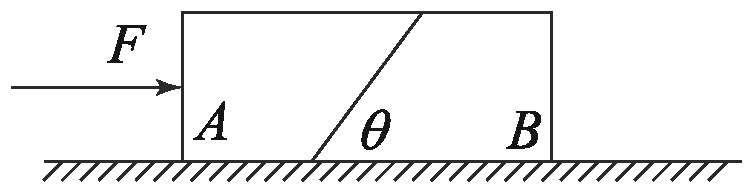
\includegraphics[width = 0.4\textwidth]{images/newton-1.pdf} 
	\end{flushright}
	\tagged{student}{\vspace*{4cm}}
	\begin{taggedblock}{teacher}
		\noindent
		解析:\[(m_A+m_B)g\mu<F<=m_Ag\tan\theta\]
		\[\tan\theta>\frac{(m_A+m_B)\mu}{m_A}\]
	\end{taggedblock}
\end{example}
%%%%%%%%%%%%%%%%%%%%%%

%%%%%%%%%%%%%%%%%
\begin{example}
	
	如图所示,质量分别为$m_{1,2}$的两个木块重叠后放在光滑的水平面上。
	两者之间的动摩擦系数为$\mu$,现给$m_1$施加随时间增大的力$F=kt$,式中$k$是常数。
	试求$m_1$和$m_2$的加速度$a_1$和$a_2$与时间的关系并画出此关系的图像。
	\begin{flushright}
		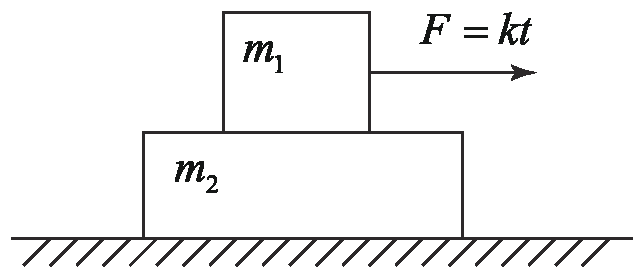
\includegraphics[width = 0.4\textwidth]{images/newton-8.pdf} 
	\end{flushright}
	\tagged{student}{\vspace*{4cm}}
	\begin{taggedblock}{teacher}
		\noindent
		解析:略
	\end{taggedblock}
\end{example}
%%%%%%%%%%%%%%%%%%%%%%


根据第一定律不受力的质点将做匀速直线运动,它的一个直接推论就是做曲线运动的质点必然要受到外力的作用。
在前面的运动学中曾经提到加速度的大小和方向与速度变化之间的关系:
\begin{enumerate}
	\item 加速度沿速度方向的分量可以用来衡量速度大小的变化率,如果用$v$表示运动质点的速速度大小,那么
	\begin{equation}
	a\cos\theta = \frac{\Delta v}{\Delta t},
	\end{equation}
	其中$\theta$为加速度和速度方向的夹角。
	\item 加速度垂直于速度的分量决定了轨迹的曲率半径
	\begin{equation}\label{key}
	\rho = \frac{v^2}{a\sin\theta}.
	\end{equation}
\end{enumerate}
在第二定律告诉我们加速度和受力之间有简单的正比例关系,可以将上面的运动学结论直接应用到动力学当中。

%%%%%%%%%%%%%%%%%%%%%%%%%%%%%%%%%%
\begin{example}
质量为$m$的质点$A$固定在长为$L$、不可变形且质量可以忽略不计的轻杆一端,杆的另一端固定在$O$点处。
杆带着质点以匀角速度$ \omega$在竖直平面上匀速转动,求$A$对杆作用力的大小和方向。
\begin{flushright}
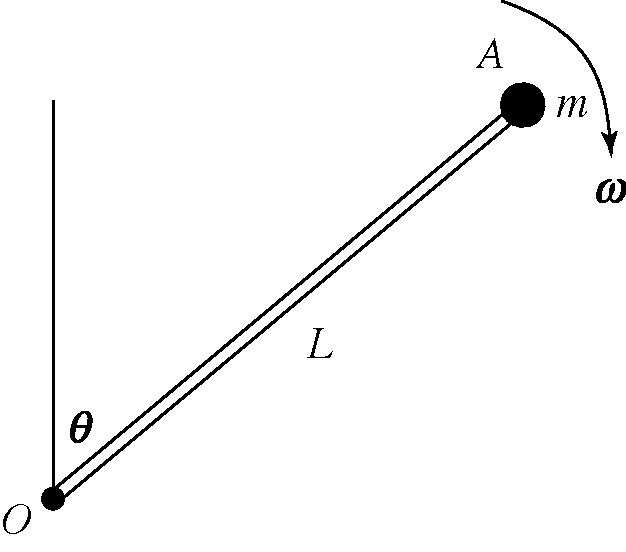
\includegraphics[width=0.3\textwidth]{images/newton-problem-2.pdf}
\end{flushright}
\tagged{student}{\vspace*{4cm}}
\begin{taggedblock}{teacher}
\noindent
解析:以向外为正方向:
\[F=m\omega^2L-mg\cos\theta\]
\end{taggedblock}
\end{example}
%%%%%%%%%%%%%%%%%%%%%%%%%%













%%%%%%%%%%%%%%%%%%
%\begin{example}
%如图,忽略一切摩擦,$A$、$B$质量为$m$,圆柱的质量为$4m$,半径为$R$。
%先用外力固定如图,在某时刻撤去外力,求圆柱落地所需要的时间。
%\begin{flushright}
%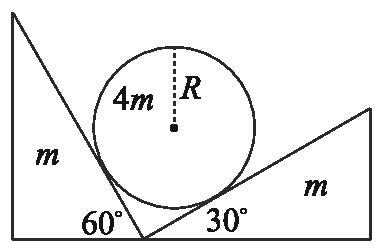
\includegraphics[width = 0.3\textwidth]{images/newton-2.pdf} 
%\end{flushright}
%
%\tagged{student}{\vspace*{4cm}}
%\begin{taggedblock}{teacher}
%\noindent
%解析:
%\end{taggedblock}
%\end{example}
%%%%%%%%%%%%%%%%%%%%%%%

%%%%%%%%%%%%%
\begin{example}
	粗糙的圆盘上放有一个质量为$m$的物体,它与圆盘之间的摩擦系数为$\mu$,与圆心的距离为$r$。
	求该物体能够与圆盘保持相对静止时圆盘围绕其中心转动的最大角速度$\omega_0$。
	\tagged{student}{\vspace*{4cm}}
	\begin{taggedblock}{teacher}
		\newline
		解析:
		\[\omega_0^2*r=\mu\]
	\end{taggedblock}
\end{example}
%%%%%%%%%%%%%%%%%%%%



%%%%%%%%%%%%%
%\begin{example}
%	赛车转弯所需要的力完全由轮胎和地面之间的摩擦力给出,当赛车高速运行时它只能够以相对较大的弧线转弯,即使这样在到达弯道前也必须适当减速。
%	最简单的假设下,轮胎和地面之间横向最大静摩擦力正比于赛车的质量,比例系数为$\mu$。
%	为使赛车用最短的时间里转弯,在下图所示的几种弯道处定性地画出赛车最佳的运行轨迹。	
%	\tagged{student}{\vspace*{4cm}}
%	\begin{taggedblock}{teacher}
%		\newline
%		解析:
%	\end{taggedblock}
%\end{example}
%%%%%%%%%%%%%%%%%%%%

当一个动力学系统包含多个物体时,它们在受力作用下的加速度大小和方向都有可能不同,这时它们之间的约束对于确定各个物体加速度的关系起着至关重要的作用。
在运动学中我们曾经学过在受约束情况下求彼此速度之间关系的方法,根据问题的特点可以采用几何、代数、微元法或其它方便的办法。
同样的问题也将出现在动力学当中,包含多个物体的动力学系统中除了受外力作用以外,那些限制各个物体的运动的连接或表面也会有力的作用,我们将这种力称之为\emph{约束力}。
对于约束的求解在很多时候非常重要,为此目的,我们必须找到彼此之间运动状态并不独立的各个物体之间加速度的关系。
我们通过以下几个例子来熟悉这类问题:


%%%%%%%%%%%%%
\begin{example}
	一个质量和摩擦均不计的定滑轮两端通过不可伸长的绳连接,绳子的一端系有质量为$m_1$的重物,另一端则有一个质量为$m_2$的同学。
	现该同学用力拉绳子使他相对于绳子以加速度$a$向上运动,求重物的加速度以绳中的张力。为使绳中的张力为零则他应当以什么样的方式运动?
	\tagged{student}{\vspace*{4cm}}
	\begin{taggedblock}{teacher}
		\newline
		解析:
		$F=m_2g+m_2a=m_1g-m_1a'$
		绳中张力为0,他应该松开绳子或以重力加速度向下运动。
	\end{taggedblock}
\end{example}
%%%%%%%%%%%%%%%%%%%%


%%%%%%%%%%%%%
\begin{example}
	如图所示,一个质量为$M_1$的物体挂在质量和摩擦均不计的定滑轮$A$的一侧,另一侧挂有一个质量为$M_2$的滑轮,它的两侧则分别挂有质量分别为$m_1$、$m_2$的两个物体。
	求$m_1$、$m_2$的加速度以及绳中的张力$T$和$T_1$。
		\begin{flushright}
			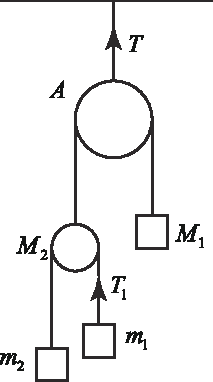
\includegraphics[width = 0.3\textwidth]{images/newton-14.pdf} 
		\end{flushright}
	\tagged{student}{\vspace*{4cm}}
	\begin{taggedblock}{teacher}
		\noindent
		解析:设M1以加速度$a_1$上升,$m_1$以$a_1-a_2$向下加速,$m_2$以$a_1+a_2$向下加速
		得到四个方程:
		\[2T_1=\frac{T}{2}\]\[
		T_1=m_1(g-a_1+a_2)\]\[
		T_1=m_2(g-a_1+a_2)\]\[
		\frac{T}{2}=M_1(a_1+g)
		\]解出:
		\[T_1=\frac{2M_1m_1m_2g}{4m_1m_2-M_1(m_1-m_2)}\]
		
	\end{taggedblock}
\end{example}
%%%%%%%%%%%%%%%%%%%%

%%%%%%%%%%%%%%%%%
\begin{example}
	
	一质量为$m$的物体放在质量为$M$,倾角为$\theta$的斜面上,两者一起放置于水平面上。
	忽略一切摩擦,求两者的加速度。
	\begin{flushright}
		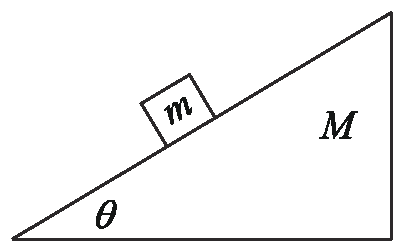
\includegraphics[width = 0.3\textwidth]{images/newton-3.pdf} 
	\end{flushright}
	\tagged{student}{\vspace*{4cm}}
	\begin{taggedblock}{teacher}
		\noindent
		解析:设M向右加速度$a_1$,m相对于M有沿斜面的加速度$a_2$
		\[(m+M)a_1=ma_2\cos\theta\]
		\[N\sin\theta=Ma_1\]
		\[mg-N\cos\theta=ma_2\sin\theta\]
		解出:
		\[a_1=\frac{mg}{\frac{m+M}{\cos\theta}+\frac{M\cos\theta}{\sin\theta}}\]
	\end{taggedblock}
\end{example}
%%%%%%%%%%%%%%%%%%%%%%

%%%%%%%%%%%%%
\begin{example}
	一根质量为$m$的杆被限制在竖直方向运动,它与一个倾角为$\theta$、质量为$M$的斜面接触,接触点的摩擦可忽略不计,不考虑斜面与水平的摩擦。
	求使斜面以加速度$a$向右运动所需要的水平外力$F$的大小。
		\begin{flushright}
			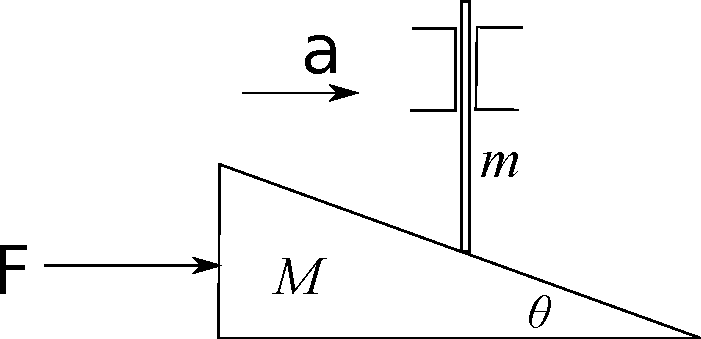
\includegraphics[width = 0.4\textwidth]{images/newton-12.pdf} 
		\end{flushright}
	\tagged{student}{\vspace*{4cm}}
	\begin{taggedblock}{teacher}
		\noindent
		解析:$F=m(g+a\tan\theta)\tan\theta$
	\end{taggedblock}
\end{example}
%%%%%%%%%%%%%%%%%%%%

\section{非惯性系中的运动}

之间我们无数次地强调牛顿定律只有在惯性参考系中才成立,那么这是否意味着在那些相对于惯性参考系,也就是所谓的非惯性参考系中物体的运动就不能够用类似的方式描写物体在受力下的加速运动规律了呢?
严格地讲是的,牛顿定律只能够在惯性参考系中成立,但其实只需要在惯性参考系中得到物体的运动方程,然后通过坐标变换就可以得到相对于非惯性系的运动方程。


考虑两个相对运动的参考系$S$和$S'$,其中$S$是一个惯性参考系,牛顿运动定律成立;$S'$是一个相对于$S$做加速度为$\vec{a_r}$的匀加速运动。
简单起见考虑一个质量为$m$的质点$P$,它受多个力的作用,这些力的合力可写为$\vec{F}$,因为$S$是一个惯性参考系,所以相对于它牛顿第二定律
\[
\vec{F} = m\vec{a}
\]
成立,其中$\vec{a}$是$P$相对于$S$的加速度。
因为$S'$与$S$的相对运动已知,根据在运动学学习过程中所掌握的规律,质点$P$相对于$S'$的加速度为$\vec{a}' = \vec{a}-\vec{a}_r$,这样如果以$S'$为参考系的话$P$的质量乘以它的加速度可以表达为:
\[
m\vec{a}' = m\vec{a}-m\vec{a}_r = \vec{F}-m\vec{a}_r。
\]
因为相对于惯性参考系,一个质量的质量乘以加速度被认为是它所受的合力,而相对于一个非惯性参考系,如果我们同样认为一个质点的质量与加速度的乘积是某种形式力的话,从中我们可以看出这个“力”并不等于合外力,而等于真实地作用于该质点的合力$\vec{F}$与$\vec{F}_i = -m\vec{a}_r$之和。

简单的推广可以发现,如果在非惯性系中存在的多个相互作用质点的话,如果假想每个质点除了受到已知的外力以及彼此之间的相互作用力以外,再加上一个假想的,正比于其质量,正比于非惯性系相对于惯性参考系的加速度$\vec{a}_r$,与非惯性系加速度方向相反的力之后,对每一个质量为$m_i$,合力为$\vec{F}_i$的质点来说它相对于非惯性系的加速度$\vec{a}_i$满足
\begin{equation}\label{key}
m_i\vec{a}_i = \vec{F}_i-m_i\vec{a}_r.
\end{equation}
这样一个假想的力被称之为\emph{惯性力},是一个由于参考系的加速运动带来的“表观力”,并不是真实存在的力,它没有施力物体,牛顿第三定律也不适用。
利用惯性力可以帮助我们以更简单的方式计算非惯性参考系中的物理过程,尤其是那种相对于非惯性参考系中所有物体均保持静止的情况,这时动力学问题被简化为一个静力学问题。

%%%%%%%%%%%%%
\begin{example}
  很多时候可以近似认为地球表面是一个惯性参考系,现有一个相对于地面以加速度$a$作匀加速度直线运动的车,车内一个质量为$m$的小球被挂在车顶,求小球相对车箱静止时悬线与竖直方向的夹角$\theta_1$。
  若将小球拉到竖直方向并由静止释放,求它摆动最高点与竖直方向的夹角$\theta_2$
  	\begin{flushright}
  		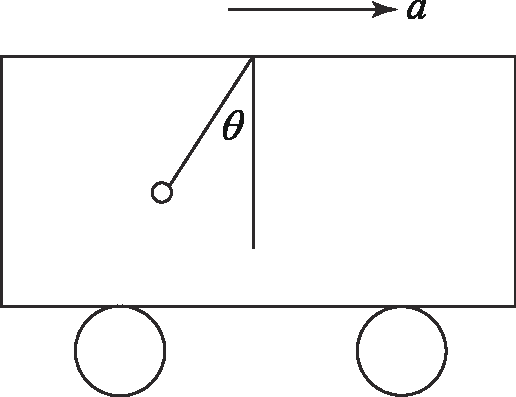
\includegraphics[width = 0.3\textwidth]{images/newton-15.pdf} 
  	\end{flushright}
	\tagged{student}{\vspace*{2cm}}
	\begin{taggedblock}{teacher}
		\noindent
		解析:$\tan\theta_1=\frac{a}{g}$
		\newline
		$\theta_2=2\theta_1$
	\end{taggedblock}
\end{example}
%%%%%%%%%%%%%%%%%%%%


%%%%%%%%%%%%%
\begin{example}
	不计空气阻力,证明在地表附近自由下落的“电梯”当中所有物体相对于电梯均做匀速直线运动。
	思考一下,在证明过程中你忽略了什么,得到了什么样的结论,这个电梯是一个惯性参考系吗?
		\begin{flushright}
			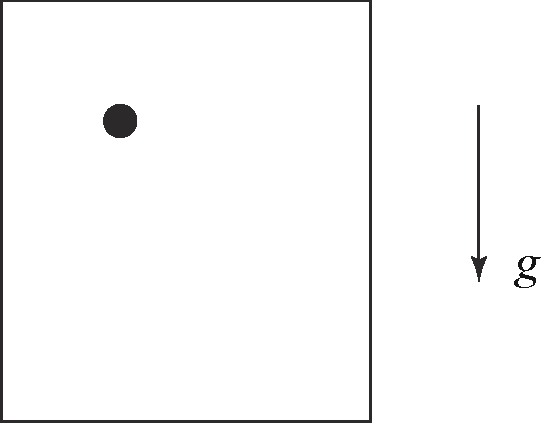
\includegraphics[width = 0.3\textwidth]{images/newton-16.pdf} 
		\end{flushright}
	\tagged{student}{\vspace*{2cm}}
	\begin{taggedblock}{teacher}
	\noindent	
		解析:略
	\end{taggedblock}
\end{example}
%%%%%%%%%%%%%%%%%%%%


%%%%%%%%%%%%%
\begin{example}
	如图所示,汽车内固定有一个倾角为$\theta$的斜面,斜面表面光滑,底部有一个质量为$ m $的小
	物块,开始时系统静止,某时刻汽车突然开始向左以加速度$a $做匀加速运动。要使物体沿斜面向上运动,则$ a $至少多大?
		\begin{flushright}
			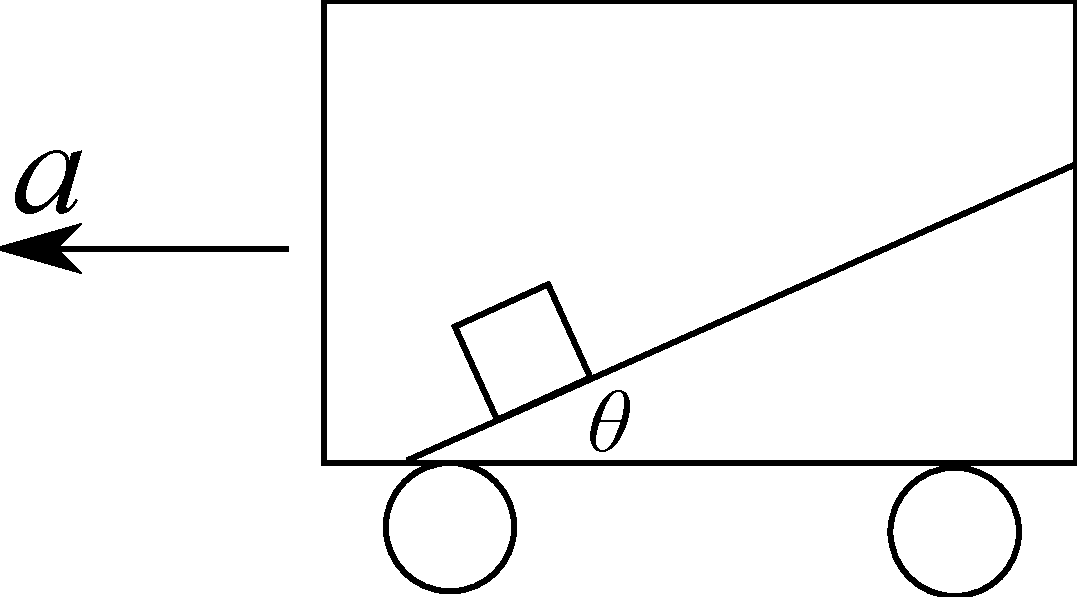
\includegraphics[width = 0.3\textwidth]{images/newton-13.pdf} 
		\end{flushright}
	\tagged{student}{\vspace*{4cm}}
	\begin{taggedblock}{teacher}
		\noindent
		解析:$a>g\tan\theta$
	\end{taggedblock}
\end{example}
%%%%%%%%%%%%%%%%%%%%


%%%%%%%%%%%%%%%%%
\begin{example}
	如图所示,在光滑水平面上有一斜面,倾角为$\alpha$,一质量为$m$的物体放在上面,在水平力$F$推动下恰使物体$m$与斜面无相对滑动,求斜面对物块弹力的大小。
	\begin{flushright}
		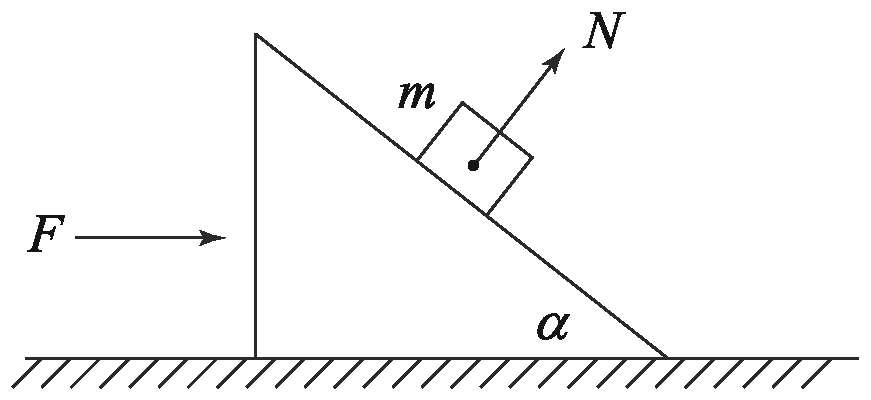
\includegraphics[width = 0.4\textwidth]{images/newton-9.pdf} 
	\end{flushright}
	
	\tagged{student}{\vspace*{4cm}}
	\begin{taggedblock}{teacher}
		\noindent
		解析:$\frac{mg}{\cos\alpha}$
	\end{taggedblock}
\end{example}
%%%%%%%%%%%%%%%%%%%%%%


%%%%%%%%%%%%%%%%%
\begin{example}
	如图所示,一个质量为$M$,两边倾角分别为$\alpha$和$\beta$的斜面放于水平面上,两个斜面上分别放有质量为$m_1$和$m_2$的物块$A$和$B$,忽略一切摩擦,求由静止释放后所有物体的加速度。
	\begin{flushright}
		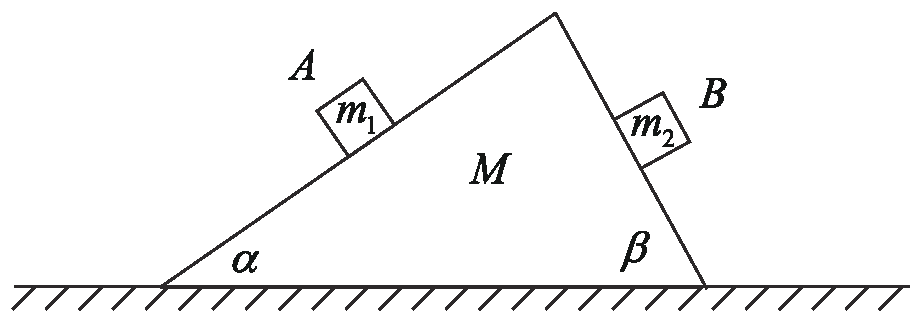
\includegraphics[width = 0.4\textwidth]{images/newton-4.pdf} 
	\end{flushright}
	
	\tagged{student}{\vspace*{4cm}}
	\begin{taggedblock}{teacher}
		\noindent
		解析:速度分解,参考3.22
	\end{taggedblock}
\end{example}
%%%%%%%%%%%%%%%%%%%%%%

%%%%%%%%%%%%%
\begin{example}
	有一个装满水的水箱当中有一个气泡,当水箱以加速度$a$向前加速运动时,那么这个气泡将$\underline{\qquad\qquad}$(向前、向后)运动。
		\begin{flushright}
			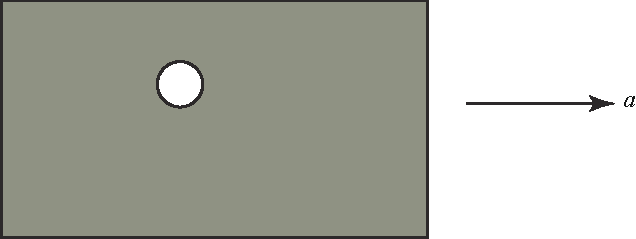
\includegraphics[width = 0.3\textwidth]{images/newton-17.pdf} 
		\end{flushright}
	\tagged{student}{\vspace*{2cm}}
	\begin{taggedblock}{teacher}
		\noindent
		解析:向前
	\end{taggedblock}
\end{example}
%%%%%%%%%%%%%%%%%%%%


如果一个物体相对于匀速转动的参考系中保持静止,那么相对于惯性参考系它将做匀速圆周运动,根据圆周运动的知识我们知道它必须受到向心力的作用。
此时在转动参考系看来它将有离开转动中心的趋势,为了使它保持相对静止就必须施加一定的外力。
简单的分析可知,当物体质量为$m$,与转轴的距离为$r$且转动参考系匀速圆周运动的角速度为$\omega$时,使质点保持相对静止所需力的大小
\begin{equation}
F = m\omega^2r,
\end{equation}
方向则是指向转动轴。
相对于转动参考系,物体保持静止,看上去上面这个力是与一个“力”在对抗并且保持“平衡”,这样一个假想的力就是我们熟悉的\emph{离心力},大小与$F$相同,方向则是沿着物体和转轴连线方向向外。

%%%%%%%%%%%%%
\begin{example}
	一根无摩擦的细杆与竖直方向的夹角为$\theta$,以恒定的角速度$\omega$匀速转动。
	杆上在距离固定中心$l$处套有一个质点在杆的转动过程中能够与它保持相对静止,求角速度$\omega$。
	
	如果物体与杆之间有摩擦,且摩擦系数为$\mu$,求能够保持相对静止角速度$\omega$的范围。
		\begin{flushright}
			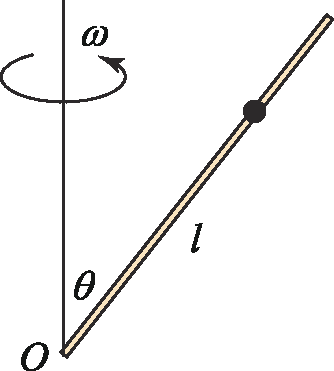
\includegraphics[width = 0.3\textwidth]{images/newton-18.pdf} 
		\end{flushright}
	\tagged{student}{\vspace*{4cm}}
	\begin{taggedblock}{teacher}
		\noindent
		解析:$m\omega^2l\sin\theta\tan\theta=mg$
		\newline
		$m\omega^2\sin\theta\tan(\theta\pm\arctan\mu)=mg$
		\end{taggedblock}
		\end{example}
		%%%%%%%%%%%%%%%%%%%%
		
%%%%%%%%%%%%%
\begin{example}
	在航空医学研究中用到的离心机,是一个绕竖直轴转动的水平杠,杠的一端携带着一个实验对象。
	如果从转动中心到实验对象的距离为$7$米,那么离心机要转动多快才能使这个乘坐者经受到$5g$的加速度?
	\tagged{student}{\vspace*{4cm}}
	\begin{taggedblock}{teacher}
		\newline
		解析:$a=\omega^2l=5g$
	\end{taggedblock}
\end{example}
%%%%%%%%%%%%%%%%%%%%



